\documentclass[12pt]{article}
\usepackage[brazil]{babel}
\usepackage[utf8]{inputenc}
\usepackage{amsmath}
\usepackage{amsfonts}
\usepackage{amssymb}
\usepackage{geometry}
\usepackage{graphicx}
\usepackage{float}
\usepackage{enumitem}
\usepackage{multicol}
\usepackage{array}
\usepackage{xcolor}

\usepackage[T1]{fontenc}
\usepackage{mathptmx} %times new roman


\geometry{a4paper, margin=1.2cm}
\setlength{\parindent}{0cm}

%\newcommand{\vermelho}[1]{{\color{red}#1}}
% implementa contador
% Definindo o contador e o comando de questão
\newcounter{questao}
\newcommand{\novaquestao}[1]{%
  \stepcounter{questao}%
  \subsection*{Questão \thequestao\ (#1)}%
}

\title{ATIVIDADE AVALIATIVA DE MATEMÁTICA}
\author{CETI BILÍNGUE GILBERTO MESTRINHO DE MEDEIROS RAPOSO}
\date{}

\begin{document}
    % Cabeçalho reduzido
    \thispagestyle{empty}
    \vspace{0.5cm}
    \begin{center}
        \large
        \begin{tabular}{|l l|}
            \hline
            \textbf{ESCOLA:} & EETI GILBERTO MESTRINHO DE MEDEIROS RAPOSO \\ 
            \textbf{ALUNA(O):} & \underline{\hspace{7cm}} \textbf{SÉRIE:} \underline{\hspace{1.5cm}} \textbf{TURMA:} \underline{\hspace{1.5cm}} \\
            \textbf{PROFESSOR:} & \underline{\hspace{7cm}} \textbf{DATA:} \underline{\hspace{1.5cm}}/\underline{\hspace{1.5cm}}/\underline{\hspace{1.5cm}} \\
            \textbf{VALOR:} & \underline{\hspace{3cm}} \textbf{NOTA:} \underline{\hspace{1.5cm}} \\
            \hline
        \end{tabular}
    \end{center}
    \vspace{0.5cm}
    
    % Título manual
    \begin{center}
        \Large\textbf{LISTA DE EXERCÍCIOS SOBRE GEOMETRIA ESPACIAL}
    \end{center}
    
    \vspace{0.3cm}
    
    \section*{ATENÇÃO:}
    \begin{itemize}[noitemsep]
        \item Resolva toda a lista, justificando cada questão.
        \item Colocar o nome completo e identificação no cabeçalho.
        \item Faça na lista, se e somente se a resolução de cada questão couber em cada questão.
        \item Há apenas uma opção correta em cada questão de múltipla escolha.
        \item Caso opte por fazer numa folha à parte, identifique cada questão.
    \end{itemize}
    % Início das colunas com linha vertical
    %\mostravermelhotrue
    \begin{multicols}{2}
        \columnseprule=0.4pt
        \columnsep=20pt
        
        \novaquestao{PSC-UFAM 2014}
            A figura a seguir é composta por uma pirâmide hexagonal regular inscrita em um prisma hexagonal regular reto. Podemos afirmar que:

            \begin{center}
                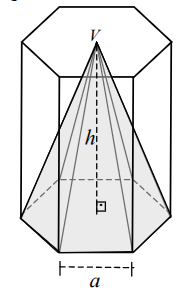
\includegraphics[scale=0.6]{imagem/q3.png}
            \end{center}
        
            \begin{enumerate}[label=(\Alph*), noitemsep]
                \item {O volume da pirâmide é um terço do volume do prisma.} %
                \item O volume do prisma é o dobro do volume da pirâmide.
                \item A área total da pirâmide é um terço da área total do prisma.
                \item A área total do prisma é um terço da área total da pirâmide.
                \item A área lateral da pirâmide é um terço da área total do prisma.
            \end{enumerate}
        
        \novaquestao{PSC-UFAM 2018}
            Na figura a seguir, o volume do sólido com vértices nos pontos A, D, E, H, G é, em $cm^{3}$:

            \begin{center}
                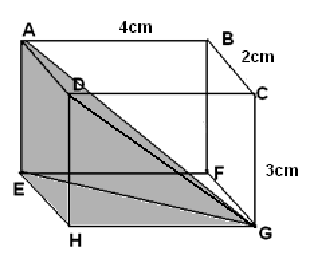
\includegraphics[scale=0.6]{imagem/q11.png}
            \end{center}
            
            \begin{enumerate}[label=(\Alph*), noitemsep]
                \item ${8}/{3}$
                \item 6
                \item {8} %
                \item 12
                \item 24
            \end{enumerate}
        
        \novaquestao{PSC-UFAM 2019}
            Sobre um tetraedro regular de aresta medindo 6 cm, é \textbf{CORRETO} afirmar que:
        
            \begin{enumerate}[label=(\Alph*), noitemsep]
                \item {Seu volume é igual a $18\sqrt{2}\ cm^{3}$} %
                \item Sua altura mede $3\sqrt{6}\ cm$
                \item O apótema da base mede $2\sqrt{3}\ cm$
                \item Sua área lateral é igual a $27\sqrt{2}\ cm^{2}$
                \item Sua área total é igual a $36\sqrt{6}\ cm^{2}$
            \end{enumerate}
        
        \novaquestao{PSC-UFAM 2021}
            Aumentando em $2\ cm$ a aresta de um cubo, sua área total aumenta em $384\ cm^{2}$. Logo, o volume do cubo original era igual a: 
        
            \begin{enumerate}[label=(\Alph*), noitemsep]
                \item $1854\ cm^{3}$
                \item $2172\ cm^{3}$
                \item $2856\ cm^{3}$
                \item {$3375\ cm^{3}$} %
                \item $4220\ cm^{3}$
            \end{enumerate}
        
        \novaquestao{PSC-UFAM 2022}
            Dois recipientes, um cilíndrico e um cônico, têm a mesma altura e bases com raios iguais. Se a capacidade do recipiente cônico é de 205 mL, então a capacidade do recipiente cilíndrico é de:
        
            \begin{enumerate}[label=(\Alph*), noitemsep]
                \item $205\ ml$
                \item $410\ ml$
                \item $505\ ml$
                \item {$615\ ml$} %
                \item $750\ ml$
            \end{enumerate}
        
        \novaquestao{PSC-UFAM 2022}
            Uma fábrica armazena seus produtos em caixas de papelão com forma de prisma reto, cujas medidas estão indicadas na figura a seguir:

            \begin{center}
                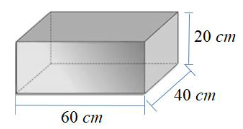
\includegraphics[scale=0.6]{imagem/q16.png}
            \end{center} Considerando que em certa semana foram usadas 10.000 dessas caixas e, desconsiderando os desperdícios, podemos afirmar que foram utilizados para confeccionar todas as caixas:
        
            \begin{enumerate}[label=(\Alph*), noitemsep]
                \item $4.400\ m^{2}$ de papelão
                \item $5.900\ m^{2}$ de papelão
                \item $6.200\ m^{2}$ de papelão
                \item $7.400\ m^{2}$ de papelão
                \item {$8.800\ m^{2}$ de papelão}%
            \end{enumerate}
    
        \novaquestao{PSC-UFAM 2023}
            Um cilindro reto possui área total igual a $32\pi\ cm^{2}$. Sabendo que o raio da base é {1}/{3} da medida da altura desse cilindro, então a área lateral desse cilindro mede:
        
            \begin{enumerate}[label=(\alph*), noitemsep]
                \item $12\pi\ cm^{2}$
                \item $18\pi\ cm^{2}$
                \item $20\pi\ cm^{2}$
                \item {$24\pi\ cm^{2}$} %
                \item $28\pi\ cm^{2}$
            \end{enumerate}

        \novaquestao{SIS - UEA 2019}
            Um prisma reto, de 8 cm de altura, tem como base um polígono de seis lados, conforme mostra a figura.
            
            \begin{center}
                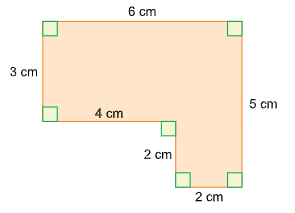
\includegraphics[scale=0.6]{imagem/q7.png}
            \end{center} O volume desse prisma é:
        
            \begin{enumerate}[label=(\Alph*), noitemsep]
                \item $160 \ cm^{3}$
                \item $168 \ cm^{3}$
                \item {$176 \ cm^{3}$} %
                \item $184 \ cm^{3}$
                \item $192 \ cm^{3}$
            \end{enumerate}

        \novaquestao{SIS-UEA 2022}
            Considere um sólido oco, com a forma de paralelepípedo reto-retângulo, contendo $1 344\  cm^{3}$ de água, com faces e arestas de espessura desprezível, em que uma das arestas mede $16\ cm$ e outra aresta mede $12\ cm$. Esse sólido está apoiado sobre uma das faces de maneira que a altura da coluna de água seja igual a $14\ cm$. A área total desse sólido é:
        
            \begin{enumerate}[label=(\alph*), noitemsep]
                \item $800\ cm^{2}$
                \item {$832\ cm^{2}$} %
                \item $864\ cm^{2}$
                \item $896\ cm^{2}$
                \item $928\ cm^{2}$
            \end{enumerate}

        \novaquestao{SIS-UEA 2023}
            Um prisma reto tem por base um pentágono com dois ângulos retos, conforme mostra a figura 1.

            \begin{center}
                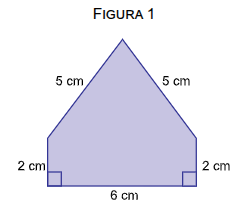
\includegraphics[scale=0.6]{imagem/q1-fig1.png}
            \end{center} O volume desse prisma é igual a $168\ cm^{3}$ e a figura 2 mostra uma vista desse prisma quando está apoiado sobre um dos pentágonos.

            \begin{center}
                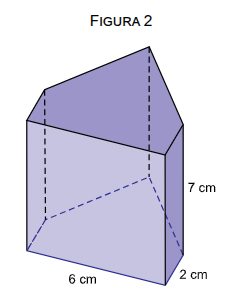
\includegraphics[scale=0.6]{imagem/q1-fig2.png} 
            \end{center} A área total desse prisma, em $cm^{2}$, é:
        
            \begin{enumerate}[label=(\alph*), noitemsep]
                \item 140
                \item 164
                \item {188} %
                \item 212
                \item 236
            \end{enumerate}

        \novaquestao{SIS-UEA 2024}
            Uma das faces de um paralelepípedo retorretângulo tem $44\ cm^{2}$ de área, sendo que nessa face a medida da maior aresta excede a medida da menor aresta em $7\ cm$. Sabendo que o volume desse paralelepípedo é $308\ cm^{3}$ , sua área total é:

            \begin{enumerate}[label=(\alph*), noitemsep]
                \item {$298\ cm^{2}$} %
                \item $336\ cm^{2}$
                \item $352\ cm^{2}$
                \item $412\ cm^{2}$
                \item $448\ cm^{2}$
            \end{enumerate}
            
        \novaquestao{MACRO-UEA 2024}
            Uma fábrica de doces faz bombons maciços de chocolate na forma de um prisma reto de base quadrada e com $1,5\ cm$ de altura, conforme mostra a figura.

            \begin{center}
                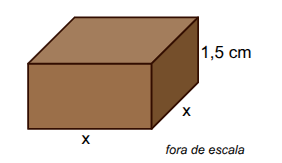
\includegraphics[scale=0.6]{imagem/q24.png}
            \end{center} Sabendo que para fabricar 85 bombons desse tipo são necessários $510\ cm^{3}$ de massa de chocolate, a medida da aresta da base, indicada na figura pela letra x, é igual a
        
            \begin{enumerate}[label=(\alph*), noitemsep]
                \item 1,5  cm
                \item 0,5  cm
                \item 2,5  cm
                \item 1,0  cm
                \item {2,0  cm} %
            \end{enumerate}

        \novaquestao{MACRO-UEA (Exatas) 2024}

            Um sólido, no formato de um cilindro circular reto, tem volume igual a $54\pi\ cm^{3}$, e sua área lateral $(A_{L})$ é calculada pela expressão $A_{L}=2\pi \times R \times H$, em que R e H são, respectivamente, o raio da base e a altura do cilindro. Sabendo que a medida da altura desse cilindro é o dobro da medida do raio da sua base, a área lateral desse cilindro, em $cm^{2}$, é:
            
                \begin{enumerate}[label=(\alph*), noitemsep]
                        \item {$36\pi$}
                        \item $27\pi$
                        \item $32\pi$
                        \item $40\pi$
                        \item $42\pi$
                    \end{enumerate}
    
        \novaquestao{ENEM 2023}
            Uma indústria de sucos utiliza uma embalagem no formato de prisma reto de base quadrada, com aresta da base de medida a e altura de medida h, ambas de mesma unidade de medida, como representado na figura.
            
            \begin{center}
                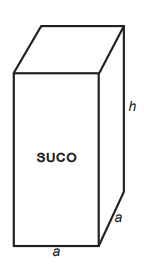
\includegraphics[scale=0.6]{imagem/q5.png}
            \end{center} Deseja-se criar uma linha de produção para uma nova embalagem de igual formato, mas que deverá ter uma capacidade igual ao triplo da atual. A altura da nova embalagem será igual a {4}/{3} da altura da embalagem atual. As arestas da base da nova embalagem serão denominadas de x. 
            Qual a relação de dependência entre a medida x da nova aresta da base e a medida a da aresta atual?
        
            \begin{enumerate}[label=(\Alph*), noitemsep]
                \item $x = a$
                \item $x = 3a$
                \item $x = 9a$
                \item {$x = 3a / 2$} %
                \item $x = a\sqrt{3}$
            \end{enumerate}

        \novaquestao{ENEM 2010}
            Uma fábrica produz barras de chocolates no formato de paralelepípedos e de cubos, com o mesmo volume. As arestas da barra de chocolate no formato de paralelepípedo medem 3cm de largura, 18cm de comprimento e 4cm de espessura. Analisando as características da figuras geométricas descritas, a medida das arestas dos chocolates que têm o formato de cubo é igual a:
            
            \begin{enumerate}[label=(\alph*), noitemsep]
                \item 5  cm
                \item {6  cm} %
                \item 12  cm
                \item 24  cm
                \item 25  cm 
            \end{enumerate}

        \novaquestao{ENEM 2010}
            Um arquiteto está fazendo um projeto de iluminação de ambiente e necessita saber a altura que deverá instalar a luminária ilustrada na figura.

            \begin{center}
                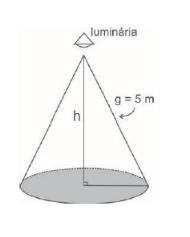
\includegraphics[scale=0.6]{imagem/q30.png}
            \end{center} Sabendo-se que a luminária deverá iluminar uma área circular de $28,26\ m^{2}$, considerando $\pi \approx 3,14$, a altura h será igual a:
        
            \begin{enumerate}[label=(\alph*), noitemsep]
                \item 3 cm
                \item {4 cm} %
                \item 5 cm
                \item 9 cm
                \item 16 cm 
            \end{enumerate}

        \novaquestao{ENEM 2010}
            Dona Maria, diarista na casa da família Teixeira, precisa fazer café para servir as vinte pessoas que se encontram numa reunião na sala. Para fazer o café, Dona Maria dispõe de uma leiteira cilíndrica e copinhos plásticos, também cilíndricos.

            \begin{center}
                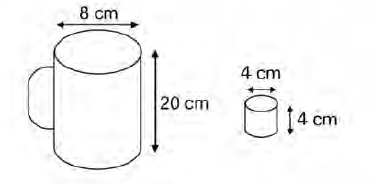
\includegraphics[scale=0.6]{imagem/q31.png}
            \end{center} Com o objetivo de não desperdiçar café, a diarista deseja colocar a quantidade mínima de água na leiteira para encher os vinte copinhos pela metade. Para que isso ocorra, Dona Maria deverá:

            \begin{enumerate}[label=(\alph*), noitemsep]
                \item {Encher a leiteira até a metade, pois ela tem um volume 20 vezes maior que o volume do copo.} \\ %
                \item Encher a leiteira toda de água, pois ela tem um volume 20 vezes maior que o volume do copo. \\
                \item Encher a leiteira toda de água, pois ela tem um volume 10 vezes maior que o volume do copo. \\
                \item Encher duas leiteiras de água, pois ela tem um volume 10 vezes maior que o volume do copo. \\
                \item Encher cinco leiteiras de água, pois ela tem um volume 10 vezes maior que o volume do copo. 
            \end{enumerate}
        

        \novaquestao{EEAR-SP 2022}
            Seja um prisma reto de 15 cm de altura. Suas bases são trapézios de 6 cm e 4 cm de base e 5 cm de altura. O volume deste prisma equivale a $ x $ vezes o volume de um cubo de aresta 5 cm. Determine $x$.
        
            \begin{enumerate}[label=(\Alph*), noitemsep]
                \item seis
                \item {três} %
                \item duas
                \item cinco
                \item sete \\
            \end{enumerate}

        \novaquestao{EEAR-SP 2021}
            A base de uma pirâmide é uma das faces de um cubo de aresta a. Se o volume do cubo somado com o volume da pirâmide é $2a^{3}$, a altura da pirâmide é x da aresta a. Esse x equivale:
        
            \begin{enumerate}[label=(\Alph*), noitemsep]
                \item ao dobro
                \item {ao triplo} %
                \item a metade 
                \item a terça parte
                \item a metade do dobro
            \end{enumerate}

        \novaquestao{UNESP-SP}
            Se $d'$ é o comprimento da diagonal da face de um cubo, então o volume desse cubo é:

            \begin{enumerate}[label=(\alph*), noitemsep]
                \item $\dfrac{\sqrt{2}}{2}(d')^{3}$ \\
                \item $\dfrac{\sqrt{2}}{4}(d')^{3}$ \\ %
                \item $\dfrac{(d')^{3}}{8}$ \\
                \item $\dfrac{(d')^{3}}{4}$ \\
                \item $(d')^{3}$
            \end{enumerate}

        \novaquestao{UTFPR-PR 2017}
            Uma barraca de camping foi projetada com a forma de uma pirâmide de altura 3 metros, cuja base é um hexágono regular de lados medindo 2 metros. Assim, a área da base e o volume da barraca medem, respectivamente:

            \begin{enumerate}[label=(\alph*), noitemsep]
                \item {$6\sqrt{3}\ m^{2}$ e $6\sqrt{3}\ m^{2}$} \\ % 
                \item $3\sqrt{3}\ m^{2}$ e $3\sqrt{3}\ m^{2}$ \\
                \item $5\sqrt{3}\ m^{2}$ e $2\sqrt{3}\ m^{2}$ \\ 
                \item $2\sqrt{3}\ m^{2}$ e $5\sqrt{3}\ m^{2}$ \\ 
                \item $4\sqrt{3}\ m^{2}$ e $8\sqrt{3}\ m^{2}$
            \end{enumerate}

        \novaquestao{UEPG - PR}
            Um caleidoscópio tem a forma de um prisma triangular regular. Sabendo-se que o apótema de sua base mede $\sqrt{3}\ cm$ e sua altura mede $18\ cm$, a área lateral mede:

            \begin{enumerate}[label=(\alph*), noitemsep]
                \item $162\sqrt{3}\ cm^{2}$ 
                \item $972\ cm^{2}$ 
                \item $108\sqrt{3}\ cm^{2}$ 
                \item {$324\ cm^{2}$} %
                \item $162\ cm^{2}$
            \end{enumerate}

        \novaquestao{E.E. Volta Redonda - RJ}
            Um prisma hexagonal regular tem aresta lateral medindo $2a\sqrt{3}$ e aresta da base mede $a$. Assim, seu volume será:

            \begin{enumerate}[label=(\alph*), noitemsep]
                \item $2\sqrt{3}a^{3}$ 
                \item $3a^{3}$ 
                \item {$9a^{3}$}  %
                \item $\sqrt{3}a^{3}$ 
                \item $\dfrac{\sqrt{3}}{2}a^{3}$
            \end{enumerate}
        
        \novaquestao{CEFET - PR}
            A diagonal do cubo cuja área total é $150\ m^{2}$ mede, em m:

            \begin{enumerate}[label=(\alph*), noitemsep]
                \item $5\sqrt{2}$ 
                \item {$5\sqrt{3}$} %
                \item $6\sqrt{2}$
                \item $6\sqrt{3}$ 
                \item $7\sqrt{2}$
            \end{enumerate}

        \novaquestao{UECE 2017}
            A medida da altura de uma pirâmide é 10 m e sua base é um triângulo retângulo isósceles cuja medida da hipotenusa é 6 m. Pode-se afirmar que a medida do volume dessa pirâmide, em $m^{3}$, é igual a:
        
            \begin{enumerate}[label=(\alph*), noitemsep]
                \item {$30$} % 
                \item $60$ 
                \item $15$  
                \item $45$  
                \item $50$
            \end{enumerate}

        \novaquestao{Poliedro-SP 2022}
            A base de um prisma reto é um pentágono regular com 1,2 m de lado. Se a altura desse sólido for de 80 cm, então sua área lateral deverá medir:
        
            \begin{enumerate}[label=(\alph*), noitemsep]
                \item $4800\ m^{2}$
                \item $480\ m^{2}$
                \item $48\ m^{2}$ 
                \item {$4,8\ m^{2}$} 
                \item $0,48\ m^{2}$
            \end{enumerate}

        \novaquestao{UFRGS 2000}
            Na figura, O é o centro do cubo.

            \begin{center}
                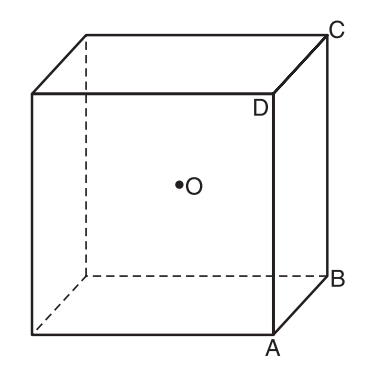
\includegraphics[scale=0.6]{imagem/qUFRS.png}
            \end{center} Se o volume do cubo é 1, o volume da pirâmide de base ABCD e vértice O é:
            
            \begin{enumerate}[label=(\alph*), noitemsep]
                \item ${1}/{2}$
                \item ${1}/{3}$
                \item ${1}/{4}$ 
                \item {${1}/{6}$} %
                \item ${1}/{8}$
            \end{enumerate}
        
        \novaquestao{UFRJ 2000}
            Considerando um lustre de formato cônico com altura e raio da base igual a $0,25$ m, a distância do chão (H) em que se deve pendurá-lo para obter um lugar iluminado em forma de círculo com área de $25\pi m^{2}$, é de:

            \begin{center}
                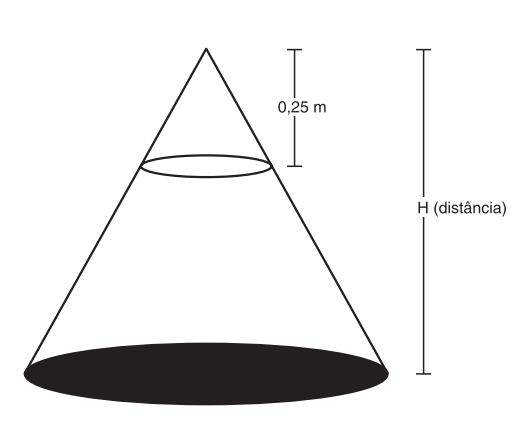
\includegraphics[scale=0.5]{imagem/UFRJ-CONE.png}
            \end{center} 
            
            \begin{enumerate}[label=(\alph*), noitemsep]
                \item 12 m
                \item 10 m
                \item 8 m
                \item 6 m
                \item {5 m} %
            \end{enumerate}

        \novaquestao{Einstein 2025}

        Na figura, estão representados o prisma retorretângulo ABCDEFGH e a pirâmide BCDL. O vértice L da pirâmide está na reta que contém a aresta $\overline{CG}$ do prisma. O prisma e a pirâmide BCDL têm o mesmo volume.

            \begin{center}
                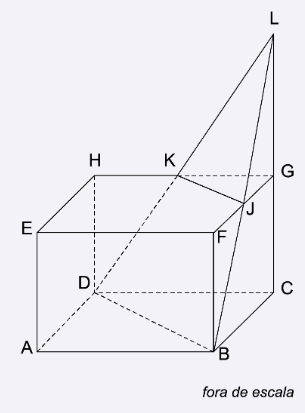
\includegraphics[scale=0.7]{imagem/einstein_2025.png}
            \end{center} O ponto J está na interseção dos segmentos $\overline{BL}$ e $\overline{FG}$, e o ponto K está na interseção dos segmentos $\overline{DL}$ e $\overline{GH}$. O volume da pirâmide GJKL, em relação ao volume do prisma, corresponde a:

         \begin{enumerate}[label=(\alph*), noitemsep]
            \item $\dfrac{125}{216}$ \\  %
            \item $\dfrac{16}{25}$ \\
            \item $\dfrac{3}{4}$ \\
            \item $\dfrac{25}{36}$ \\
            \item $\dfrac{64}{125}$ 
        \end{enumerate}

        \novaquestao{Livro}

            Para calcular a capacidade de um jarro de forma irregular, Paulo retirou água de um aquário que tem a forma de um paralelepípedo retorretângulo e encheu completamente o jarro.

            \begin{center}
                
\includegraphics[scale=0.5]{imagem/paiva-aquario.png}
            \end{center} Observando que o fundo do aquário tem 50 cm de
            comprimento por 30 cm de largura e que, após a
            retirada, o nível da superf ície da água desceu 2 cm,
            o rapaz concluiu, corretamente, que a capacidade
            do jarro é:

            \begin{enumerate}[label=(\alph*), noitemsep]
                \item $3\ L$ %
                \item $0,3\  L$
                \item $2\ L$
                \item $2,8\ L$
                \item $2,7\  L$
            \end{enumerate}

        \novaquestao{Fuvest 2006}

            A partir de 64 cubos brancos, todos iguais, forma-se um novo cubo. A seguir, este novo cubo tem cinco de suas seis faces pintadas de vermelho.

            \begin{center}
                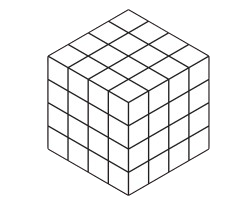
\includegraphics[scale=0.7]{imagem/fuvest-cubo.png}
            \end{center} O número de cubos menores que tiveram pelo menos duas de suas faces pintadas de vermelho é:

            \begin{enumerate}[label=(\alph*), noitemsep]
                \item 24 %
                \item 26
                \item 28
                \item 30
                \item 32
            \end{enumerate}

        \novaquestao{Ulbra - RS}

        	Sabendo-se que cada degrau tem a forma e as dimensões do prisma a seguir, o volume de concreto que se gasta para fazer 10 degraus é:

            \begin{center}
                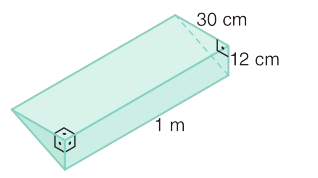
\includegraphics[scale=0.6]{imagem/ulbra-rs.png}
            \end{center}

            \begin{enumerate}[label=(\alph*), noitemsep]
                \item $0,18\ m^{3}$ %
                \item $1,8\ m^{3}$
                \item $3\ m^{3}$
                \item $18\ m^{3}$
                \item $10\ m^{3}$
            \end{enumerate}
            
           \novaquestao{Livro}
           
           		
    			As medidas das três arestas de um paralelepípedo retângulo são diretamente proporcionais a 4, 5 e 8 e a soma dessas medidas é 68 cm. O volume desse paralelepípedo, em $cm^{3}$, corresponde a qual das alternativas abaixo?
    			
    			\begin{enumerate}[label=(\alph*), noitemsep]
    				\item 10.240 %
    				\item 1024
    				\item 102
    				\item 77
    				\item 10
    			\end{enumerate}
    			
    			
    			
    \end{multicols}
    
\end{document}